\documentclass[thesis]{thesis}
\usepackage[python,linenum]{mypackage}

\title{Taichi图形库的剖析与应用}
\author{吴坎$^\star$\qquad 陈鸿峥$^\star$\qquad 戴钊煌}
\school{数据科学与计算机学院\quad 计算机类\\超算17341163,大数据17341015,超算17341027}
\authorremark{\textbf{名字排序不代表贡献大小},具体分工如下:
吴坎负责具体代码实现及统筹规划;
陈鸿峥负责论文报告撰写及PPT修改;
戴钊煌负责PPT制作及意见讨论。
由于使用中文撰写论文,故排版样式未参照IEEE/ACM的论文模板,而参照国内的期刊标准。
择选的论文为Yuanming Hu, Tzu-Mao Li, Luke Anderson, Jonathan Ragan-Kelly, Fr\'edo Durand, \emph{Taichi: A Language for High-Performance Computation on Spatially Sparse Data Structures}, SIGGRAPH Asia, 2019.}

\begin{document}
	
\maketitle
	
\begin{abstractchinese}
随着计算机图形学的不断发展,越来越多复杂的算法被提出。
传统采用OpenGL进行编程的方式,对于现在某些复杂算法来说,已显得十分低效。
因此越来越多研究者尝试将基本的图形操作算子进行进一步封装,提供更加高层次的接口,从而提升程序员的生产力。
而太極(Taichi)图形库正是这样的尝试,它主要针对图形学中常见的层次化数据结构,提出了对应的领域特定编程语言(Domain-Specific Language, DSL)和编译器。
它开创性地将图形学算法中的计算部分和数据结构部分进行解耦,一方面利于程序员更快地部署和维护复杂的数据结构,另一方面通过编译器优化又可以高效地将同一个算法部署到CPU或者GPU上,最终实现性能、可编程性和可移植性三者的权衡,大大推动了图形学研究者的算法开发过程。
本文首先对图形库及领域特定编程语言的发展状况进行阐述,然后对Taichi语言的特性进行一定讨论,最后通过自己实施算法,实现简单的实例程序并进行展示。
\end{abstractchinese}
\begin{keywordchinese}
计算机图形学,物理过程模拟,领域特定编程语言,领域特定编译器
\end{keywordchinese}

\section{简介}
从上个世纪60年代计算机图形学(Computer Graphics, CG)一词被提出来,图形学一直在不断发展焕发新的活力。
发展至今,图形学已经成为一门独立的学科,涉及数学、物理、光学、材料等等多学科的知识。
早期图形学研究者们因为资源限制,侧重研究如何在计算机中表示各种各样的图形;而随着计算机底层架构的不断发展,计算力的不断提升,图形学研究者们也愈发追求富有震撼力的视觉效果,提出了大量复杂的模拟算法。
为了更加逼真地模拟现实,做出有现实感、逼真的CG图像与视频,研究者们常常需要实现几百甚至上千行代码,才能实现一个看似很简单的功能。
这导致图形学的代码实现往往会存在一定的技术壁垒,某种程度上拖慢了现在图形学的发展速度。

现在最为常用的图形库为OpenGL\cite{opengl},发展至今将近快30年时间。
OpenGL采用C/C++进行编写,提供了大量底层画图调用接口,为开发者提供了强有力的工具去实现各种各样的视觉效果。
但由于太过底层,很多时候CG开发者们并不需要这么多功能,或者不想重复编写简单的图形变换操作,所以后来又有freeglut\cite{freeglut}、glfw\cite{glfw}、glew\cite{glew}等大量OpenGL的扩展库出现。
这些扩展库将常用的OpenGL操作进一步封装,给开发者更加高层的编程接口,使得编程效率得到很大提升。

而到2010年以后,学术界希望进一步提升语言抽象能力的同时,又保证其实施的高效性,因此产生了大量的领域特定编程语言(Domain-Specific Language)和编译器。
最典型的如Halide\cite{ragan-kelley_halide_2013}专门针对图像处理管线提出了高层编程接口,同时利用自动循环优化等技术提升代码的局部性,从而实现图像处理性能的大幅提升。
Liszt\cite{zachary_liszt_2011}是专门用于优化物理模拟过程,GraphIt\cite{yunming_graphit_2018}则是面向有限元分析等图处理的DSL。
Tiramisu\cite{riyadh_cgo_2019}是专门针对复杂嵌套循环的基于多面体技术的编译器,Taco\cite{fredrik_taco_2017}则是专门针对张量处理设计的领域特定编译器。
再到今年,MIT的几位研究人员发现在3D图形学应用中存在大量的层次化数据结构,因此他们提出了太極(Taichi)\cite{hu_taichi_2019}这一面向计算机图形学的领域特定语言,专门针对这些应用进行特定优化。

本文将着重对Taichi图形库进行深入剖析,并利用Taichi自己实现一些简单的视觉呈现。
第\ref{sec:bg}节阐述Taichi图形库的背景与动机,第\ref{sec:method}节将会介绍Taichi的核心方法学,第\ref{sec:exp}节给出我们的实验环境及实验结果,最后第\ref{sec:summary}节总结全文。


\section{背景与动机}
\label{sec:bg}
在现在的很多3D物理过程模拟中,需要大量应用层次化的数据结构来表达数据。
包括流体模拟、粒子模拟、材料特性模拟等,都是通过在不同的层次嵌套哈希表、静态数组、动态数组、指针数组等来表示数据。

图\ref{fig:nested}给出了一个层次化嵌套的数据结构的例子。
其中最顶层为\verb'Root'结构体,其中存储了$16\times 16$个\verb'Block'结构体数组;
而每个\verb'Block'又包含两个成员,一个为$16\times 16$的\verb'ChildNode'结构体静态数组,另一个为动态的\verb'child2'数组。
\begin{figure}[htbp]
\centering
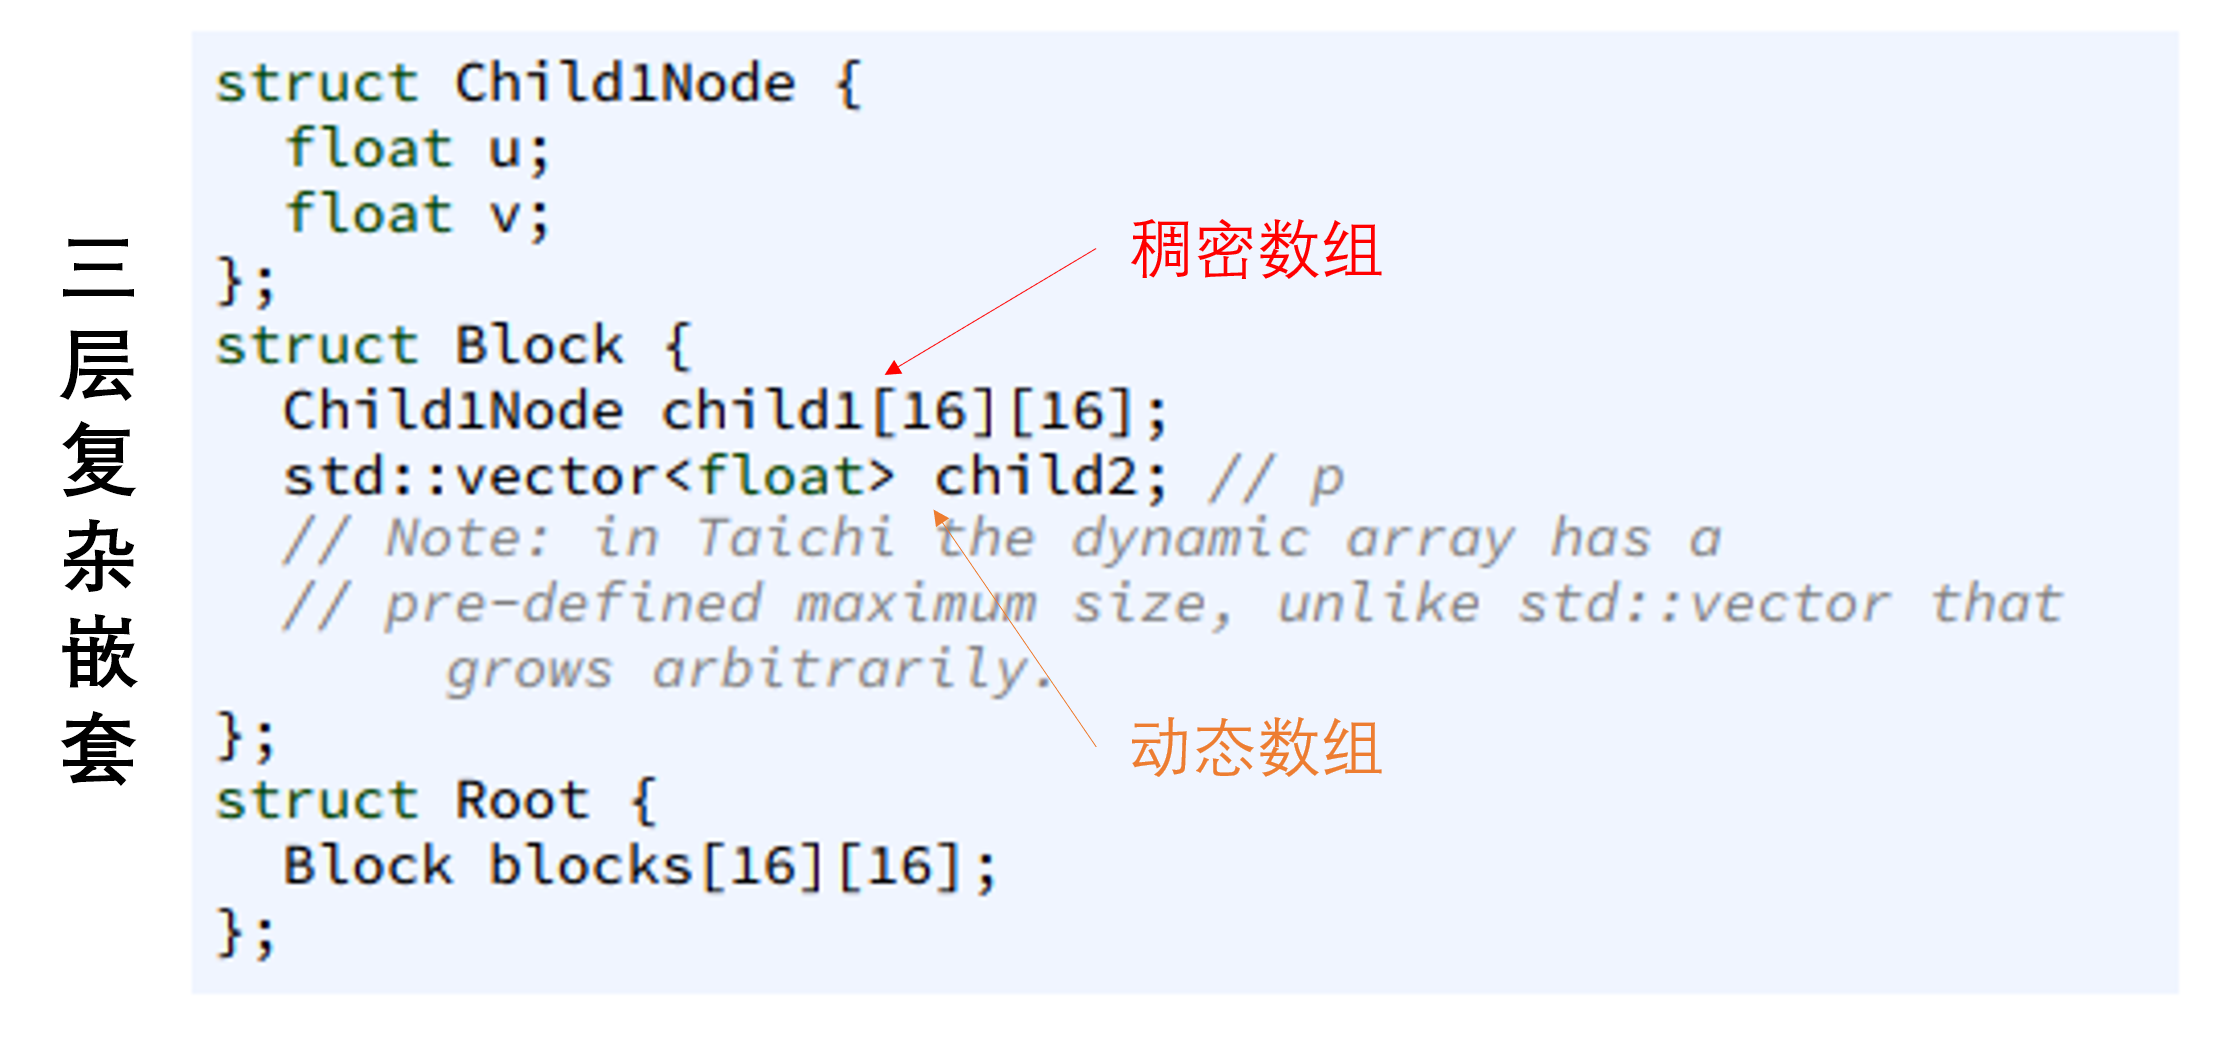
\includegraphics[width=0.6\linewidth]{fig/nested.png}
\caption{层次化嵌套数据结构}
\label{fig:nested}
\end{figure}

这只是三层的层次结构,若在每次计算中都要访问叶结点的$(u,v)$元素,在代码编写和实际运行上都已经非常麻烦。
从这一个例子中我们可以总结出这种多层嵌套的数据结构存在的挑战:
\begin{enumerate}
	\item[1)] \underline{简单地遍历层次数据结构会产生大量的冗余访存}:因为核心数据是存储在叶结点$(u,v)$上,因此每次计算访问或更新数据都不得不通过前面的父节点数据结构而访问到子节点。
	建立多个结构体只是为了符合面向对象编程的标准,使得程序员更好地组织代码,但事实上中间数据结构的访问对实际执行没有任何益处,因此这些冗余访存的开销都可以通过编译器优化抹平。
	\item[2)] \underline{难以充分利用数据局部性以发挥现代计算机体系结构的优势}:层次化数据结构的访问相当于不规则的访问,每次都需要间接索引地址,因此数据局部性非常差,导致难以充分利用现代计算机中的高速缓存。
	如果结合Stencil\cite{stencil}等本身就很复杂的数据依赖关系,那么程序运行的性能将会变得更加糟糕。
	\item[3)] \underline{难以在不同硬件上实现高效的并行}:为了适配不同的体系结构,应用研究者通常要对不同的硬件,如CPU/GPU编写不同的优化代码,以实现最大的性能。但这种方法是低效且不通用的,对于这种3D网格算法更加如此,本身就很难并行,还要部署到不同设备上,只会使问题难上加难。
\end{enumerate}

因此,Taichi图形库的提出就是为了解决以上的挑战。
通过高效实现层次化数据结构,并结合领域特定编译器优化,实现平均$4.5$倍的性能提升。
通过从数据结构中分离计算单元,提供C/C++接口以及Python的绑定,帮助程序员用$1/10$的代码量就实现同样的功能。
通过实现不同的编译器后端,使得代码可以一次编写,多次部署在不同硬件上。
最终成功实现了性能(performance)、生产力(productivity)、可移植性(portability)三者的权衡与统一。

\section{核心方法}
\label{sec:method}
本节中将按照Taichi原始论文\cite{hu_taichi_2019}的章节顺序简要介绍Taichi图形库的核心特性。

\subsection{语言特性}
Taichi DSL的核心思想是将\textbf{计算}和\textbf{数据结构}解耦。

在原始的C/C++程序中计算过程与数据结构是紧耦合的,意味着修改数据结构的同时,也要求计算过程进行相应的修改,进而编译器难以做相关的优化。
而当这两者分离后,程序员在定义数据结构时将轻松很多,同时可以将计算过程与底层存储方式隔离,实现算法的通用性。

如下面的2维离散Laplace算子
\begin{equation}
u_{i,j}=\frac{1}{\Delta x^2}(4v_{i,j}-v_{i+1,j}-v_{i-1,j}-v_{i,j+1}-v_{i,j-1})
\end{equation}
如果应用在复杂的网格结构中将会非常麻烦,所有关于$v$的访问都会带上复杂的结构名称体前缀。
而Taichi采用的方法如图\ref{fig:decouple}所示,当计算内核与数据结构相分离后,代码的编写将会变得异常简单。
两者相互不影响,而整合的过程只需交由编译器完成。
\begin{figure}[htbp]
\centering
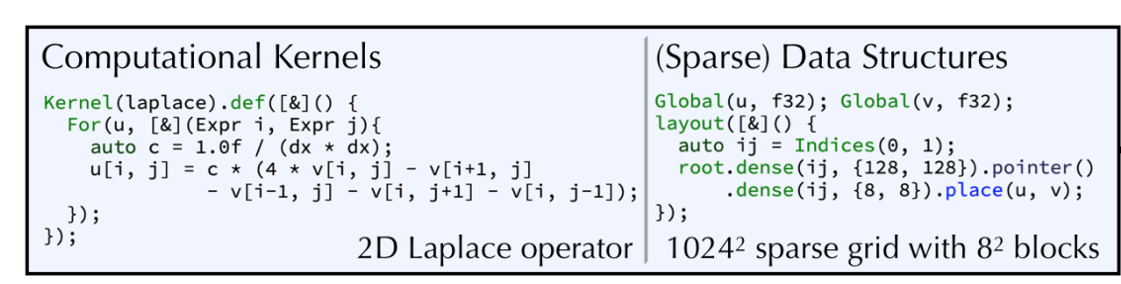
\includegraphics[width=0.6\linewidth]{fig/decouple.png}
\caption{计算内核与数据结构相分离}
\label{fig:decouple}
\end{figure}

\textbf{计算内核}类似于GPU的CUDA编程,采用Single-Program-Multiple-Data (SPMD)的方式进行编写。
只需在\verb'Kernel.def'中用C++11的Lambda表达式定义好计算过程即可。

而\textbf{数据结构}只需指定根结点\verb'root',然将下面的数据结构后逐层堆积上去即可。
Taichi提供了稠密(\verb'dense')、哈希(\verb'hash')和动态(\verb'dynamic')三种子结点类型,又提供了Z形(\verb'morton')、位掩码(\verb'bitmasked')和指针(\verb'pointer')三种结点排布方式,基本上涵盖了所有层次化数据结构。

\subsection{编译优化技术}
Taichi的编译器主要从以下三个方面优化并提升整体性能。
\begin{enumerate}
	\item [1)] \underline{提升缓存局部性}:通过边界推断(boundary inference)确定所需片上cache空间,更好地管理数据存储,也避免了过多无效的计算。
	\item [2)] \underline{删除冗余访问}:通过分析计算核在不同迭代轮次之间的重叠区域,推断计算一个块所需的内存大小,生成对应得暂存器和共享内存空间,从而利用数据的时空局部性,分摊遍历格点的成本(如图\ref{fig:opt}(a)所示)。
	\item [3)] \underline{自动并行化和任务管理}:由于网格存在稀疏性,并不是所有网格的叶子结点都需要进行计算,因此直接对叶子结点采用并行机制会导致负载不均(如图\ref{fig:opt}(b)所示)。
	Taichi采取的方法是,将数据结构展开成一维数组,再做均匀划分。
	在CPU上通过OpenMP并行处理任务队列,在GPU上则维护多个任务列表,从根节点层层生成,进而实现每个计算单元的负载近似相同。 
\end{enumerate}
\begin{figure}[htbp]
\centering
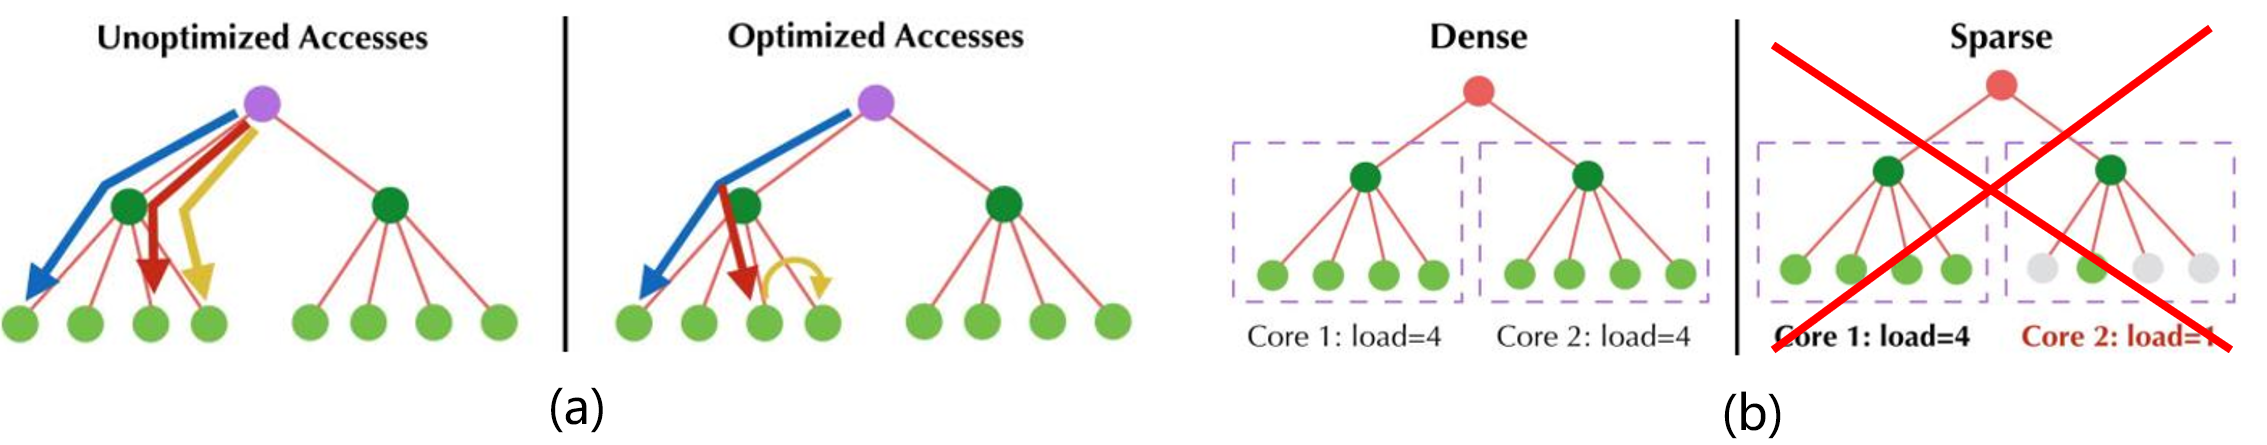
\includegraphics[width=\linewidth]{fig/opt.png}
\caption{编译器优化技术:(a) 删除冗余访问;(b) 稠密与稀疏结点任务划分对比}
\label{fig:opt}
\end{figure}

其他编译器优化技术如公共子表达式消除、局部变量存储转发、死指令消除等在此不再赘述。

\subsection{运行时优化技术}
由于用户在编写代码时可以直接跳过层次数据结构,直接访问到最底层叶子结点的数据,因此就需要编译器将用户请求的下标,转换为对应的物理地址。
这里Taichi实现了一个内存分配器,按需分配每个计算核的资源,并且实现虚拟地址空间到物理空间的映射。

CPU上除了采用常见的并行方式外,Taichi也使用了SIMD的方式,利用SSE或AVX指令集,实现多数据的并行读取与写入。

\section{实验}
\label{sec:exp}
本节会给出我们的实验环境、以及我们自己利用Taichi图形库编写的一些程序及结果。

\subsection{实验环境}
我们在VAIO Z Flip 2016的主机上进行了实验,其中有一个Intel Core i7-6567U CPU (3.30GHZ),一个核心显卡Intel Iris 550,配备8G内存。
操作系统为Windows 10的子系统Ubuntu 18.04.2 LTS,并安装了Python 3.7.4及相应的依赖库文件。
下列所有程序都使用Taichi图形库提供的Python Binding进行编程。

\subsection{实验结果}
我们充分利用Taichi图形库的特性,编写了5个图形学程序并在机器上实际运行比较结果,其中2个为官方所给的测试样例,其他的3个程序均为我们自己实现,详情细节可见下面分析。

\subsubsection{官方示例}
为测试太极环境的正常安装,我们进行基本的环境测试。
运行官方提供的太极图(运行方式可见附录\ref{appendix:env}),可正常生成如图\ref{fig:taichi}所示的图片,说明Taichi图形库正常安装并可运行。
\begin{figure}[htbp]
\centering

\includegraphics[width=0.3\linewidth]{fig/taichi.jpg}
\caption{太极图实例\protect\footnotemark}
\label{fig:taichi}
\end{figure}
\footnotetext{源代码来自:\url{https://github.com/yuanming-hu/taichi/blob/master/examples/taichi_logo.py},可见作业文件夹code/taichi\_logo,图片中呈现的为本机运行的效果。}

接着,我们尝试运行动态画面,同样运行Taichi代码库中example的例子,其流体效果如图\ref{fig:fluid}所示。
由于采用CPU进行计算,因此帧率会比较低,但是不影响正常的运行。
\begin{figure}[!ht]
\centering
\begin{tabular}{ccc}
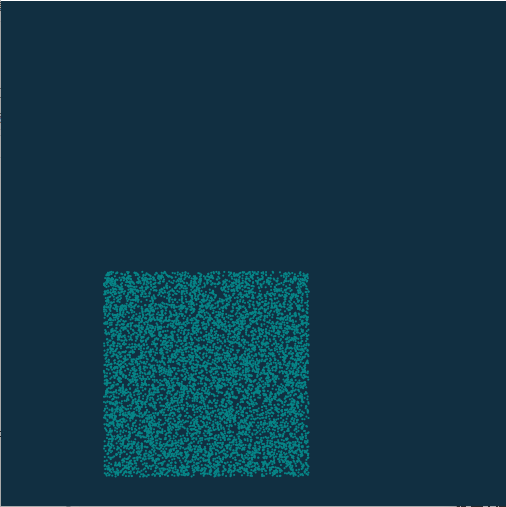
\includegraphics[width=0.33\linewidth]{fig/mpm1.png}&
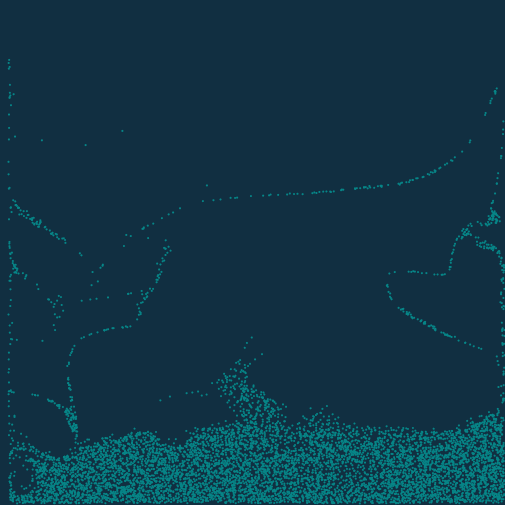
\includegraphics[width=0.33\linewidth]{fig/mpm2.png}&
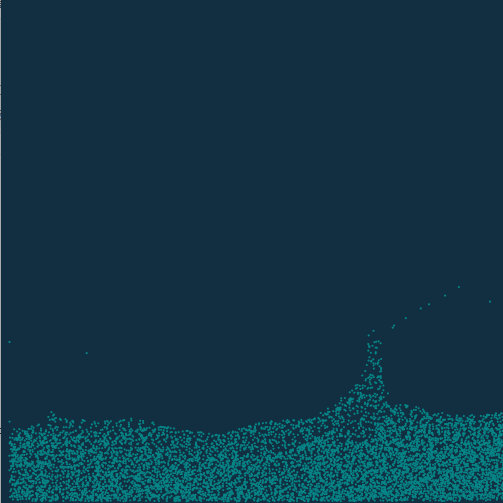
\includegraphics[width=0.33\linewidth]{fig/mpm3.png}
\end{tabular}
\caption{流体图实例\protect\footnotemark}
\label{fig:fluid}
\end{figure}
\footnotetext{源代码来自:\url{https://github.com/yuanming-hu/taichi/blob/master/examples/mpm88.py},可见作业文件夹code/mpm88,图片中呈现的为本机运行的效果。}

\subsubsection{旋转字母}
接下来的实验则全部由我们自己手写,通过学习Taichi图形库的基本语法和向量表达,我们成功实现了一些简单的图形效果。

首先第一个实验,我们渲染了SYSU四个英文字母,并使用复数乘法实现了简单的旋转效果,关于这个实验的一些细节说明如下:
\begin{itemize}
    \item 预处理阶段在CPU上生成SYSU四个像素字母,同时计算好初始坐标,送入Taichi预定义的数据结构\verb'ti.Vector'中\footnote{Taichi图形库在python导入简写为ti};
    \item 通过\verb'@ti.kernel'定义核函数,注意核函数里所有的规则循环都会被送入GPU做并行化处理;
    \item 进一步,可以类似定义\verb'@ti.func'为更细粒度的算子(比如在本实验中是\verb'complexMul'),方便核函数调用。
\end{itemize}

图\ref{fig:sysu}展示了我们自己手写的SYSU标志效果,代码可见附录\ref{appendix:sysu}或者\verb'code/sysu'文件夹。
\begin{figure}[!ht]
\centering
\begin{tabular}{ccc}

\includegraphics[width=0.33\linewidth]{fig/sysu1.jpg}&
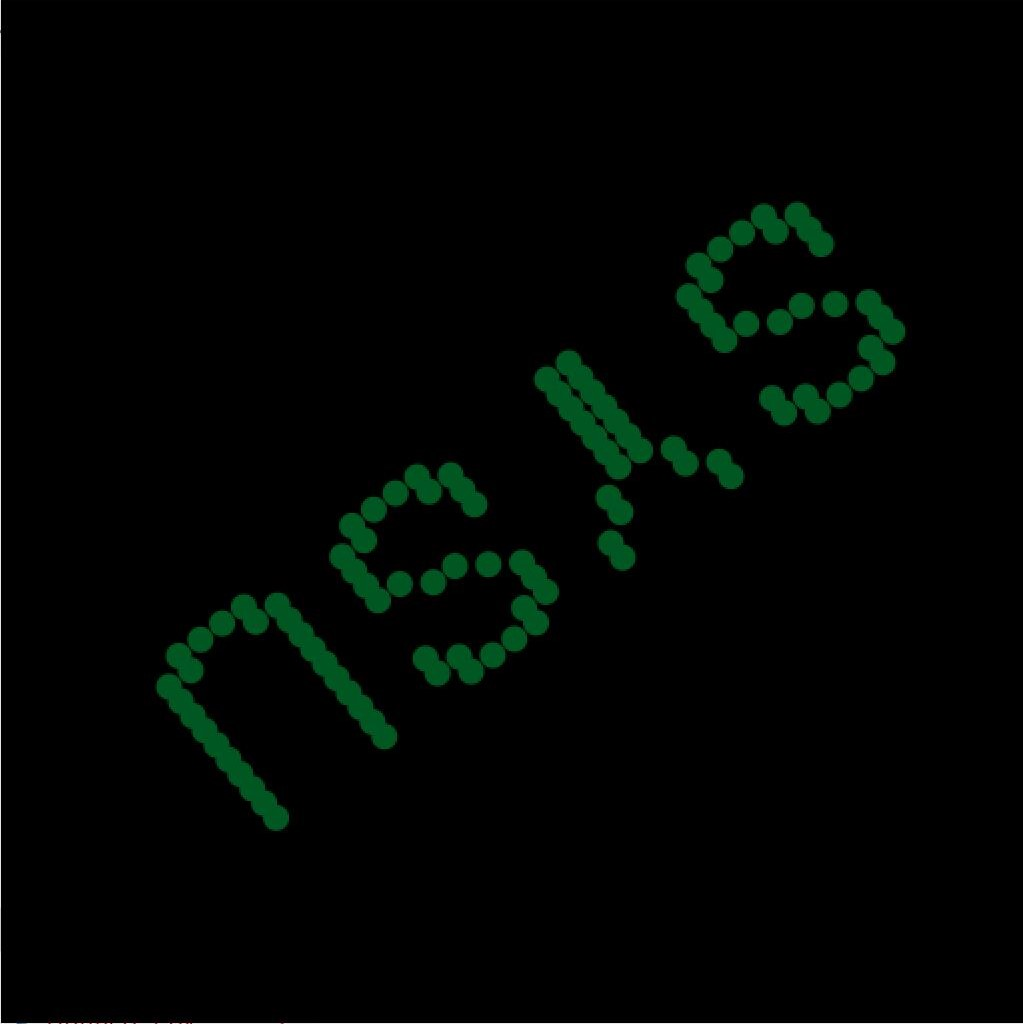
\includegraphics[width=0.33\linewidth]{fig/sysu2.jpg}&
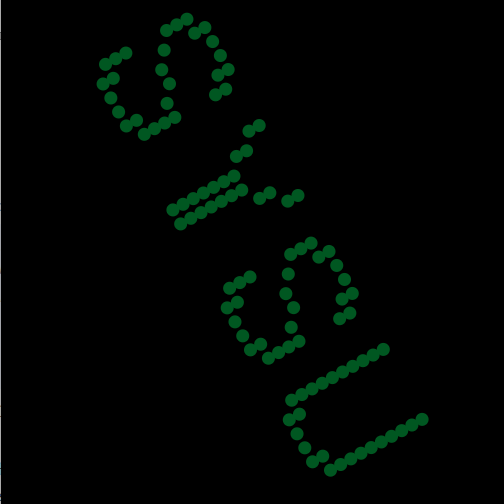
\includegraphics[width=0.33\linewidth]{fig/sysu3.png}
\end{tabular}
\caption{SYSU变换图}
\label{fig:sysu}
\end{figure}

这个实验看似简单,但是其中却蕴含着深刻的学问。
首先\textbf{代码编写}确实简单了很多,不需要繁琐地对OpenGL进行预处理,也不需要调用其他一些辅助的图形库(如GLU或GLUT等)进行矩阵计算,Taichi提供了大量矩阵/张量编程的接口,可以方便快捷地部署程序。

从\textbf{运行时间}上来看,利用Taichi图形库的实现比用Python的OpenGL裸实现的快了将近10倍,这一方面是由于Python的解释执行远不及Taichi部分使用AOT的编译执行;另一方面则是由于GPU的大规模并行带来的效果。
这里我们十分聪明地采用了细粒度的编程(有点类似于顶点着色器的思想),将每一个像素点看成是一个作用单元,然后通过在Taichi的kernel内建立for循环,对每一个像素点元进行复数乘法旋转变换。
这种方式其实正契合了GPU的SPMD的计算模式,每个核执行的都是非常小量的简单操作,但有大量成百上千个核一起算,故速度就提上去了,这也是为什么Taichi图形库能够充分利用GPU的特性为图形应用进行加速的原因。

\subsubsection{网格生成}
第二个实验我们则重新用Taichi图形库实现了作业五的内容,进一步比较其与OpenGL的区别。

由于Taichi并不提供太多的显示及控制接口,因此画面的输出显示依然采用OpenGL进行渲染。
obj文件的读入我们创建了一个\verb'Polyhedron'的类进行语法解析及处理,最终得到顶点和面的坐标,均以Python内置列表形式存储。
接下来的操作则由Taichi图形库接管:
\begin{itemize}
    \item 我们采用了Taichi最新提出的技术---面向对象数据编程(Objective data-oriented programming, ODOP)\footnote{该技术随着Taichi v0.3.8进行发布(2019年12月23日),注意到该方法官方文档尚未完善,因此我们是通过其给出的实例进行学习,并举一反三运用到我们的实验中。},将核心的网格\verb'Coord3Ds'类用\verb'@ti.data_oriented'进行封装,在初始化时将Python内置列表全部转换为Taichi图形库的向量形式进行存储。
    \item 在\verb'Coord3Ds'中,我们定义了四个核函数:
    \begin{itemize}
        \item \verb'assign':对GPU参数进行传递
        \item \verb'output_to':对GPU上计算完后的结果返回输出
        \item \verb'rotate':采用顶点着色器的编程方法,对每个顶点都进行旋转变换
        \item \verb'normal':同样对每一个顶点进行归一化处理
    \end{itemize}
    所有类中的核函数用\verb'@ti.classkernel'进行修饰,进而可以编译到GPU上并行执行。
    同时注意所有的函数传递都需要添加类型提示(type hint),以方便编译器的优化处理,其中也用到了模板元编程的思想,进一步提升泛化能力。
    \item 前面定义的是计算核,后面将定义数据结构的摆放方式。
    我们定义了\verb'place'函数并用\verb'@ti.layout'进行修饰,声明我们的3D网格结构是根(root)节点下的一个子节点。
    同时,我们也在\verb'Coord3Ds'中定义数据存放方式为稠密型存储(dense)。
\end{itemize}

图\ref{fig:mesh}展示了我们用Taichi图形库实现的多边形网格效果,具体代码可见附录\ref{appendix:mesh}或者\verb'code/cow'文件夹。
\begin{figure}[!ht]
\centering
\begin{tabular}{ccc}
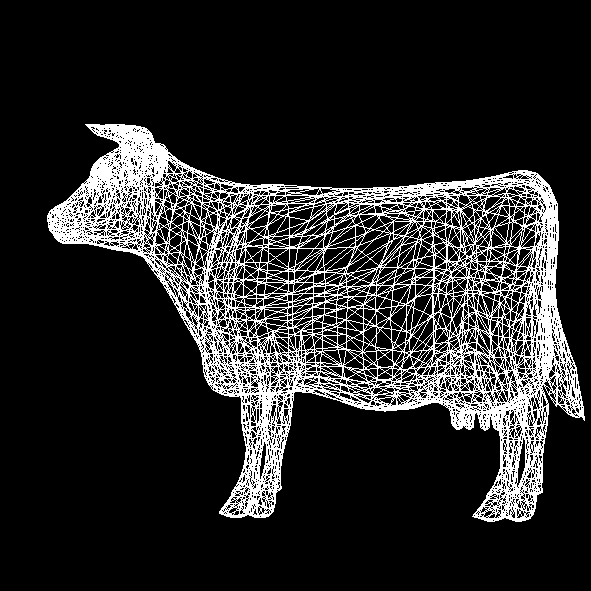
\includegraphics[width=0.33\linewidth]{fig/cow1.png}&
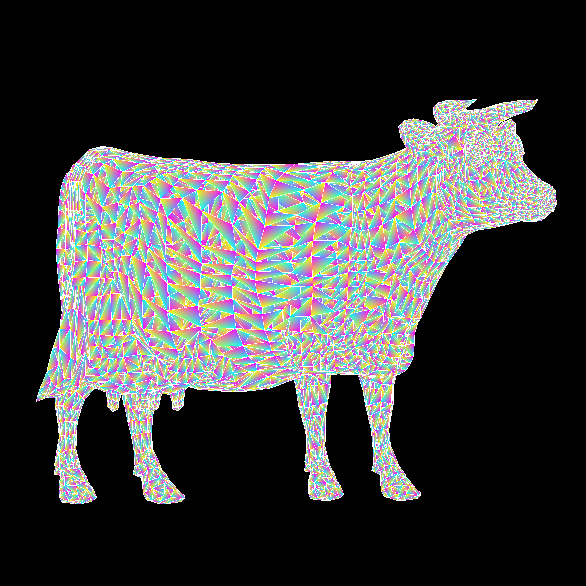
\includegraphics[width=0.33\linewidth]{fig/cow2.png}&
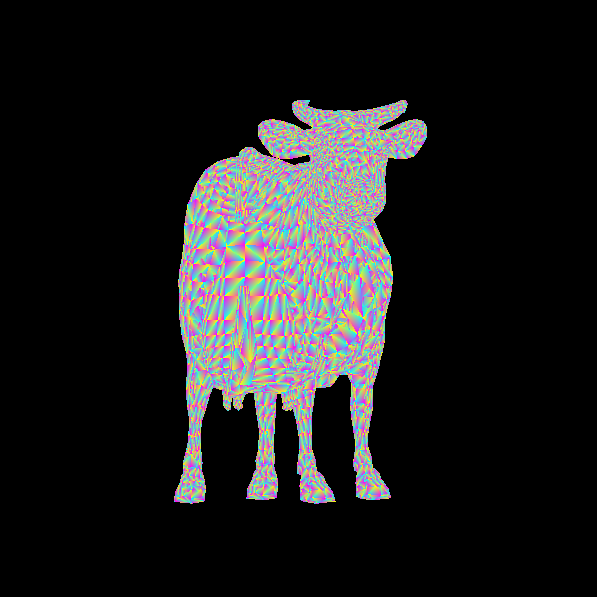
\includegraphics[width=0.33\linewidth]{fig/cow3.png}
\end{tabular}
\caption{网格生成\protect\footnotemark}
\label{fig:mesh}
\end{figure}

从上述过程中我们也可以看到,Python下的Taichi图形库处理还是快捷很多,核心的Python代码只有几十行,而当时我们完成作业五都要写上百行的代码才可以实现相应的功能。
这一个实验虽然不是典型的计算密集型应用,但是我们也从中看到Taichi图形库的核心思想---\textbf{计算与数据结构解耦}---带来的好处,程序员在编写程序时不用再关心底层的数据结构到底应该怎么定义,而可以着重于关注计算过程怎么实现,通过编译器的优化,就可以高效地将这两者结合起来。

\subsubsection{可微计算}
最后,我们实现了作者今年关于可微图形库DiffTaichi\cite{hu_difftaichi_2019}中的一个样例---可微高地场浅水水波模拟,具体论文可参见\cite{wang:wave_2018}。
由于Taichi图形库的作者在\cite{hu_difftaichi_2019}的附录E.4中已经将详细过程描述得很清楚,因此我们直接对照其更新公式进行实现。

浅水高度场(shallow water height field)水波主要依据下面这条微分方程进行模拟
\begin{equation}
\ddot{u}=c^{2} \nabla^{2} u+c \alpha \nabla^{2} \dot{u}
\end{equation}
其中$u$是浅水的高度,$c$是音速($340m/s$),$\alpha$为阻尼因子。

依据\cite{wang:wave_2018}的方法,可将上述方程采用有限不同时间域(finite different time-domain, FDTD)的方法进行离散化,并得到更新公式
\begin{equation}
\label{equ:fdtd}
u_{t, i, j}=2 u_{t-1, i, j}+\left(c^{2} \Delta t^{2}+c \alpha \Delta t\right)\left(\nabla^{2} u\right)_{t-1, i, j}-p_{t-2, i, j}-c \alpha \Delta t\left(\nabla^{2} u\right)_{t-2, i, j}
\end{equation}
其中
\begin{equation}
\label{equ:laplace}
\left(\nabla^{2} u\right)_{t, i, j}=\frac{-4 u_{t, i, j}+u_{t, i, j+1}+u_{t, i, j-1}+u_{t, i+1, j}+u_{t, i-1, j}}{\Delta x^{2}}
\end{equation}
为拉普拉斯算子(即二阶梯度的离散形式)。

其目标是最小化损失函数
\begin{equation}
L=\sum_{i,j}\Delta x^2(u_{T,i,j}-\hat{u}_{i,j})^2
\end{equation}
$T$为最大时间步,$\hat{u}$为目标高度场。
原文中采用Taichi图像作为目标高度场$\hat{u}$,而在我们实验中则使用了Project 1使用的erythrocyte动漫图像作为目标(见图\ref{fig:erythrocyte},在实际实验中我们只取图像的第1个通道作为输入)。
然后通过梯度下降,可以不断令$u$趋于$\hat{u}$,最终达到拟合效果。
\begin{figure}[!ht]
\centering

\includegraphics[width=0.33\linewidth]{fig/erythrocyte.png}
\caption{动漫图像Erythrocyte}
\label{fig:erythrocyte}
\end{figure}

所有的图片输入输出都采用python的cv2库实现,初始的一些变量初始化矩阵采用numpy库实现。
之后则是Taichi图形库的核心操作:
\begin{enumerate}
    \item 数据结构定义:同样采用\verb'@ti.place'对\verb'place'函数进行修饰。
    从上述的更新公式中我们知道在计算中会使用到四个变量
    \begin{itemize}
        \item \verb'u'、\verb'u_hat':即对应着公式\ref{equ:fdtd}中的$u$和$\hat{u}$
        \item \verb'res':用来存储中间变量
        \item \verb'loss':用来存储损失
    \end{itemize}
    因此我们只需在根结点下放置如下四个数据结构即可,代码如下。
    由于都为稠密数组,故均用\verb'dense'模式声明,同时声明\verb'grad'成员,表明需要梯度。
\begin{lstlisting}
@ti.layout
def place():
    ti.root.dense(ti.l, max_steps).dense(ti.ij, n).place(u)
    ti.root.dense(ti.l, max_steps).dense(ti.ij, n).place(u.grad)
    ti.root.dense(ti.ij, n).place(u_hat)
    ti.root.dense(ti.ij, n).place(u_hat.grad)
    ti.root.dense(ti.ij, n).place(res)
    ti.root.dense(ti.ij, n).place(res.grad)
    ti.root.place(loss)
    ti.root.place(loss.grad)
\end{lstlisting}
    \item 计算核定义:依据前面给出的公式,我们可以定义以下四个计算核
    \begin{itemize}
        \item \verb'fdtd':对照公式(\ref{equ:fdtd})
        \item \verb'laplace':对照公式(\ref{equ:laplace})
        \item \verb'initialize':初始\verb'u'数组初始化(时间步为$0$)
        \item \verb'apply_grad':梯度更新
    \end{itemize}
\end{enumerate}

由于Taichi具备自动微分功能,故我们只需直接在\verb'apply_grad'模块调用\verb'.grad'成员,并依据常见的梯度下降更新公式
\begin{equation}
\vx = \vx - lr \cdot \nabla\vx
\end{equation}
进行更新即可,其中$lr$为学习率或步长。

总结来说,我们只需在一开始通过cv2库读入图片,将其转为矩阵形式传入Taichi图形库,调用\verb'ftdt'算子,并在每一轮迭代后更新梯度,便可以完美实现该算法。
完整代码可见附录\ref{appendix:diff_wave}或者\verb'code/erythrocyte'文件夹。

实验结果如图\ref{fig:difftaichi}所示,可以看到在一轮迭代中水波的变化模式。
这是第79轮迭代的效果,已经可以从中看见我们所想要的模式了。
完整的变化视频也可以在代码文件夹中找到。
\begin{figure}[!ht]
\centering
\begin{tabular}{ccc}
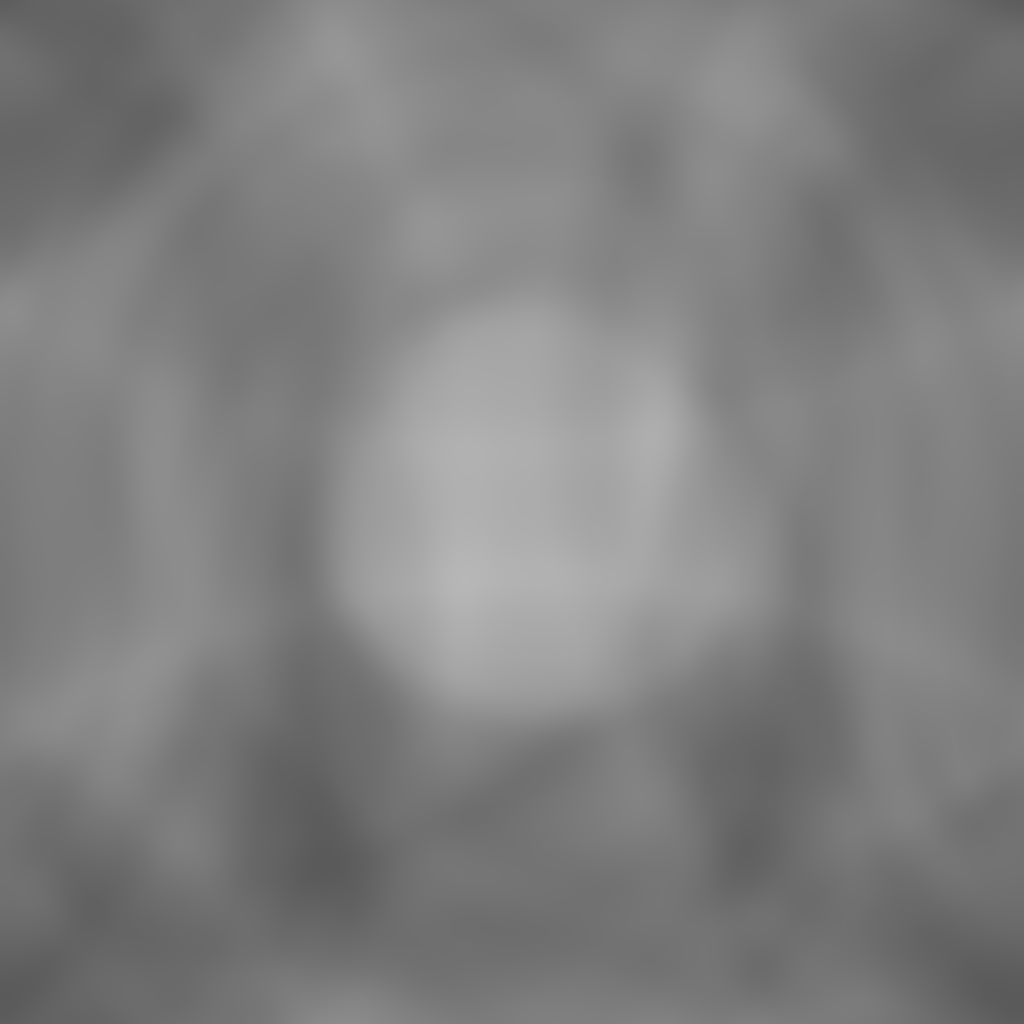
\includegraphics[width=0.33\linewidth]{fig/erythrocyte1.png}&

\includegraphics[width=0.33\linewidth]{fig/erythrocyte2.png}&
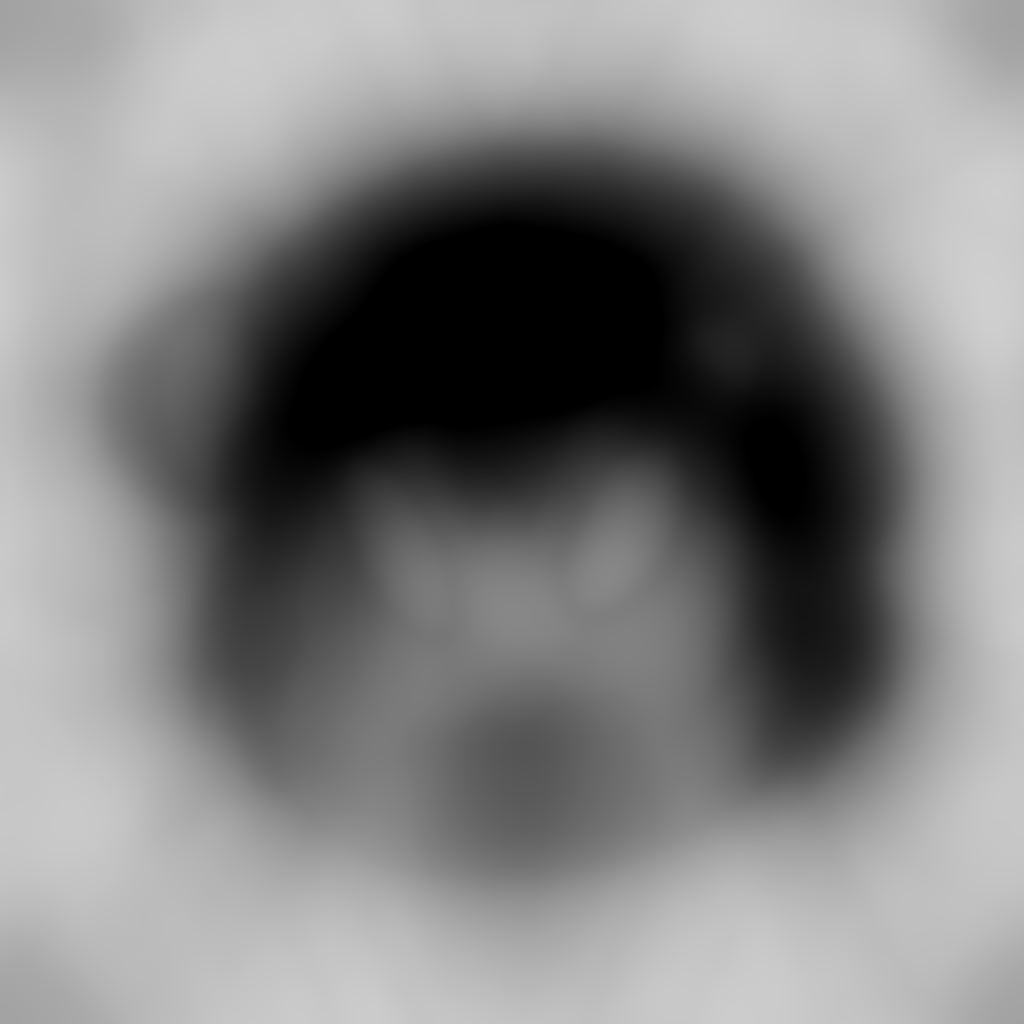
\includegraphics[width=0.33\linewidth]{fig/erythrocyte3.png}
\end{tabular}
\caption{可微高地场浅水水波模拟}
\label{fig:difftaichi}
\end{figure}

迭代过程中的损失函数变化如图\ref{fig:loss}所示,可以看到损失符合我们预期,在不断下降。
\begin{figure}[H]
\centering
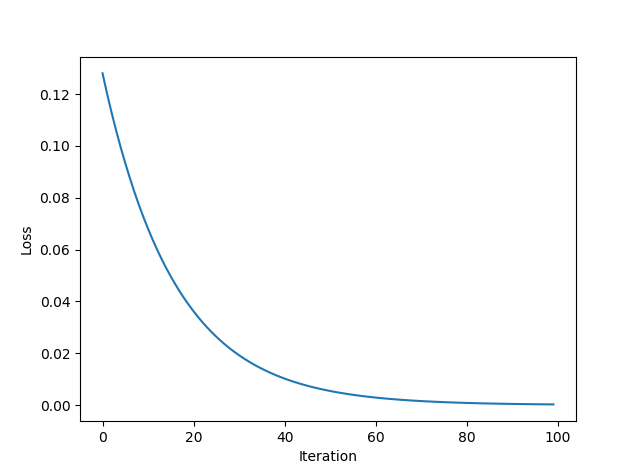
\includegraphics[width=0.5\linewidth]{fig/loss.png}
\caption{损失函数变化}
\label{fig:loss}
\end{figure}

这个实验进一步说明了Taichi图形库的优越之处,哪怕我们对\cite{wang:wave_2018}的工作不是很了解,但是通过作者在\cite{hu_difftaichi_2019}中简单叙述的几条更新公式,我们就可以快速将图形学算法进行实现,这在传统的OpenGL开发中是根本不可能的。
并且数据结构与算法相分离也给程序员带来了很大的便利,每次实施时只需关注一个点,然后将其实现即可,而复杂的交互过程全部都交由编译器实现了。
这里也不得不说Taichi图形库的编译器实现得非常的好,我们在实现中基本没有报太多的错误,并且有错误的地方也能够清晰地定位出来。

当然,在实现中我们也遇到了一些问题。
比如初次编写核函数时未考虑到GPU并行的特性,直接对loss函数进行更新,然后产生数据不一致现象。
后来才在Taichi的文档中找到了\verb'atomic_add'函数,以确保更新操作的原子性。
还有是具体实施中我们始终没有办法实现\cite{hu_difftaichi_2019}连贯的动画效果,即便在图片输出上我们已经参照了一些样例代码,但仍存在帧率太低等问题。
不过不管怎样,我们最终还是将这一前沿的图形学算法实现了(而且编码部署时间非常快),更加深刻体会到Taichi的强大之处。

\section{总结}
\label{sec:summary}
本文对常用的图形库及领域特定语言进行了一定简介,然后介绍了Taichi产生的由来与动机,接着介绍了Taichi图形库的核心特性,最后我们在自己的机器上完成了一些实验,包括Taichi内置的两个实验,以及我们自己手写的三个实验,并最终都跑出了预期的效果。

总的来看,Taichi图形库的出现大大提升了程序员的生产力,其可微编程版本更是将其应用领域扩展到更为广阔的范围。
Taichi图形库高度的抽象让图形学从业者可以更加关注于算法细节,而不是复杂的数据结构摆放及索引,可以算是近年来图形学计算库的集大成者,极大推动了图形学算法研究的发展。

\bibliographystyle{unsrt}
\bibliography{reference}

\newpage
\appendix
\appendixconfig
\section{环境配置}
\label{appendix:env}
\begin{lstlisting}[language=bash]
# CPU only. No GPU/CUDA needed. (Linux, OS X and Windows)
python3 -m pip install taichi-nightly

# With GPU (CUDA 10.0) support (Linux only)
# python3 -m pip install taichi-nightly-cuda-10-0

# execution
python3 sysu.py
\end{lstlisting}

\section{SYSU代码}
\label{appendix:sysu}
\begin{lstlisting}
import taichi as ti


def getX():
    logo = [[
        "  ####  ",
        " ##  ## ",
        " #    # ",
        " #      ",
        "  #     ",
        "   ##   ",
        "     ## ",
        " #    # ",
        " #    # ",
        " ##  ## ",
        "  ####  "
    ], [
        " #    # ",
        " #    # ",
        "  #  #  ",
        "  #  #  ",
        "   ##   ",
        "   ##   ",
        "   ##   ",
        "   ##   ",
        "   ##   ",
        "   ##   ",
        "   ##   "
    ], [
        "  ####  ",
        " ##  ## ",
        " #    # ",
        " #      ",
        "  #     ",
        "   ##   ",
        "     ## ",
        " #    # ",
        " #    # ",
        " ##  ## ",
        "  ####  "
    ], [
        " #    # ",
        " #    # ",
        " #    # ",
        " #    # ",
        " #    # ",
        " #    # ",
        " #    # ",
        " #    # ",
        " #    # ",
        " ##  ## ",
        "  ####  "
    ]]
    x = []
    for i in range(len(logo)):
        for X in range(len(logo[i])):
            for Y in range(len(logo[i][X])):
                if logo[i][X][Y] == '#':
                    x.append([i/len(logo)+Y/len(logo[i][X])/len(logo),
                              0.5+0.5/len(logo)-X/len(logo[i])/len(logo)])
    return x


ti.cfg.arch = ti.cuda
x_logo = getX()
n_particles = len(x_logo)
dim = 2
spin = [ti.cos(0.1), ti.sin(0.1)]
x = ti.Vector(dim, dt=ti.f32, shape=n_particles)
for i in range(n_particles):
    x[i] = x_logo[i]


@ti.func
def complexMul(a: ti.f32, b: ti.f32, c: ti.f32, d: ti.f32):  # `复数乘法,用于旋转'
    return [a*c-b*d, b*c+a*d]


@ti.kernel
def substep():
    for p in x:
        x[p] = x[p]-0.5
        x[p] = complexMul(x[p][0], x[p][1], spin[0], spin[1])
        x[p] = x[p]+0.5


gui = ti.core.GUI("SYSU_CG_COURSE", ti.veci(512, 512))
canvas = gui.get_canvas()
for frame in range(19260817):
    substep()

    canvas.clear(0)
    pos = x.to_numpy(as_vector=True)
    for i in range(n_particles):
        canvas.circle(ti.vec(pos[i, 0], pos[i, 1])).radius(
            7).color(87*256+33).finish()  # `中大绿'
    gui.update()
\end{lstlisting}


\section{多边形网格代码}
\label{appendix:mesh}
\begin{lstlisting}
from OpenGL.GL import *
from OpenGL.GLU import *
from OpenGL.GLUT import *
import taichi as ti
ti.cfg.arch = ti.cuda  # Run on GPU by default


class Polyhedron:
    def __init__(self, obj=None, ply=None, off=None):
        self.v = []
        self.faces = []
        if obj != None:
            for line in open(obj, 'r').readlines():
                s = line.strip().split()
                if (s[0] == "v"):
                    self.v.append([float(s[1]), float(s[2]), float(s[3])])
                elif (s[0] == "f"):
                    # `OBJ下标从1开始的,这里做转换'
                    self.faces.append([int(s[1])-1, int(s[2])-1, int(s[3])-1])


model = Polyhedron(obj='cow.obj')


@ti.data_oriented
class Coord3Ds:
    def __init__(self, n):
        self.n = n
        self.v = ti.Vector(3, dt=ti.f32)

    def place(self, root):
        root.dense(ti.i, self.n).place(self.v)

    @ti.classkernel
    def assign(self, v: ti.template()):
        for i in self.v:
            self.v[i] = v[i]

    @ti.classkernel
    def output_to(self, v: ti.template()):
        for i in self.v:
            v[i] = self.v[i]

    @ti.classkernel
    def rotate(self, c: ti.template(), d: ti.template()):
        for i in self.v:
            self.v[i][0], self.v[i][2] = self.v[i][0]*c - \
                self.v[i][2] * d,  self.v[i][2]*c+self.v[i][0]*d

    @ti.classkernel
    def normal(self):  # `归一化'
        ma = self.v[0][0]
        mi = self.v[0][0]
        for i in self.v:
            for j in ti.static(range(3)):
                ma = max(ma, self.v[i][j])
                mi = min(mi, self.v[i][j])
        for i in self.v:
            for j in ti.static(range(3)):
                self.v[i][j] = (self.v[i][j] - mi) / (ma - mi)*2-1


global_v = Coord3Ds(len(model.v))


@ti.layout
def place():
    # Place an object. Make sure you defined place for that obj
    ti.root.place(global_v)
    ti.root.lazy_grad()


v = ti.Vector(3, dt=ti.f32, shape=len(model.v))
for i in range(len(model.v)):
    v[i] = model.v[i]

global_v.assign(v)
global_v.normal()
global_v.output_to(v)
typeNum = 0


def keyboard(key, w, h):
    global typeNum
    if (key == b'r'):
        global_v.rotate(ti.cos(0.1), ti.sin(0.1))
        global_v.output_to(v)
    elif (key == b'e'):
        typeNum = (typeNum + 1) % 3
    else:
        return
    glutPostRedisplay()


def display():
    glClear(GL_COLOR_BUFFER_BIT | GL_DEPTH_BUFFER_BIT)
    glMatrixMode(GL_MODELVIEW)
    glLoadIdentity()
    for i in range(len(model.faces)):
        p0 = v[model.faces[i][0]]
        p1 = v[model.faces[i][1]]
        p2 = v[model.faces[i][2]]
        if (typeNum != 1):
            glBegin(GL_LINES)
            glColor3f(1, 1, 1)
            glVertex3f(p0[0], p0[1], p0[2])
            glVertex3f(p1[0], p1[1], p1[2])
            glVertex3f(p0[0], p0[1], p0[2])
            glVertex3f(p2[0], p2[1], p2[2])
            glVertex3f(p1[0], p1[1], p1[2])
            glVertex3f(p2[0], p2[1], p2[2])
            glEnd()
        if (typeNum != 2):
            glBegin(GL_TRIANGLES)
            glColor3f(0, 1, 1)
            glVertex3f(p0[0], p0[1], p0[2])
            glColor3f(1, 0, 1)
            glVertex3f(p1[0], p1[1], p1[2])
            glColor3f(1, 1, 0)
            glVertex3f(p2[0], p2[1], p2[2])
            glEnd()
    glFlush()


if __name__ == "__main__":
    glutInit()
    glutInitDisplayMode(GLUT_RGB | GLUT_SINGLE)
    glutInitWindowSize(600, 600)
    glutInitWindowPosition(100, 100)
    glutCreateWindow("CG_PRJ2")
    glClearColor(0, 0, 0, 0)
    glShadeModel(GL_SMOOTH)
    glutDisplayFunc(display)
    glutKeyboardFunc(keyboard)
    glutMainLoop()
\end{lstlisting}

\section{可微高地场浅水水波模拟代码}
\label{appendix:diff_wave}
\begin{lstlisting}
import cv2
import numpy as np
import taichi as ti
import matplotlib.pyplot as plt

ti.cfg.arch = ti.cuda  # Run on GPU by default
output_every = 2

# some constants
n = 256 # grid size
steps = 256
max_steps = 512

c = 340 # speed of sound
alpha = 0.00000
dx = 1 / n
inv_dx = 1 / dx
dt = (np.sqrt(alpha ** 2 + dx ** 2 / 3) - alpha) / c
learning_rate = 1

# firstly declare the variables
u = ti.var(dt=ti.f32)
u_hat = ti.var(dt=ti.f32)
res = ti.var(dt=ti.f32)
loss = ti.var(dt=ti.f32)

@ti.layout
def place():
    ti.root.dense(ti.l, max_steps).dense(ti.ij, n).place(u)
    ti.root.dense(ti.l, max_steps).dense(ti.ij, n).place(u.grad)
    ti.root.dense(ti.ij, n).place(u_hat)
    ti.root.dense(ti.ij, n).place(u_hat.grad)
    ti.root.dense(ti.ij, n).place(res)
    ti.root.dense(ti.ij, n).place(res.grad)
    ti.root.place(loss)
    ti.root.place(loss.grad)

@ti.kernel
def initialize():
    for i in range(n):
        for j in range(n):
            u[0, i, j] = res[i, j]

@ti.func
def laplace(t, i, j):
    return ti.sqr(inv_dx) * (-4 * u[t, i, j] + u[t, i, j - 1] + u[t, i, j + 1] + u[t, i + 1, j] + u[t, i - 1, j])


@ti.kernel
def fdtd(t: ti.i32):
    """
    The update formula comes from the paper DiffTaichi
    """
    for i in range(n):
        for j in range(n):
            u[t, i, j] = 2 * u[t - 1, i, j] \
                       + (ti.sqr(c) * ti.sqr(dt) + c * alpha * dt) * laplace(t - 1, i, j) \
                       - u[t - 2, i, j] \
                       - c * alpha * dt * laplace(t - 2, i, j)

@ti.kernel
def cal_loss(t: ti.i32):
    for i in range(n):
        for j in range(n):
            # make sure the atomicity when updating the same value in parallel
            ti.atomic_add(loss, ti.sqr(dx) * ti.sqr(u_hat[i, j] - u[t, i, j]))

@ti.kernel
def apply_grad():
    # gradient descent
    for i, j in res.grad:
        res[i, j] -= learning_rate * res.grad[i, j]

def forward():
    initialize()
    for t in range(2, steps):
        fdtd(t)
        # the following output framework references from Taichi examples
        if (t + 1) % output_every == 0:
            img = np.zeros(shape=(n, n), dtype=np.float32)
            for i in range(n):
                for j in range(n):
                    img[i, j] = u[t, i, j] + 0.5
            img = cv2.resize(img, fx=4, fy=4, dsize=None)
            cv2.imshow('img', img)
            cv2.waitKey(1)
            img = np.clip(img, 0, 255)
            cv2.imwrite("output/{:04d}.png".format(t), img * 255)
    cal_loss(steps - 1)

def main():
    """
    Differentiable programming framework can be found in
    https://taichi.readthedocs.io/en/latest/syntax.html#kernels
    """
    # read in figures
    img = cv2.imread('erythrocyte.png')[:,:,0]
    # normalization
    img = img / 255.0
    img -= img.mean()
    img = cv2.resize(img, (n, n))
    for i in range(n):
        for j in range(n):
            u_hat[i, j] = float(img[i, j])

    losses = []
    for it in range(100):
        # encapsulate loss in taichi
        with ti.Tape(loss):
            forward()
        print('Iter {} Loss = {}'.format(it,loss[None]))
        losses.append(loss[None])
        # update gradient
        apply_grad()

    # output loss curve
    plt.set_xlabel("Iteration")
    plt.set_ylabel("Loss")
    plt.plot(losses)
    plt.show()


if __name__ == '__main__':
    main()
\end{lstlisting}

\end{document}